% !TEX root =  manuscript.tex
\section{Prior Work}\label{sec:related}

To the best of our knowledge, 
there are no existing surveys or systematic literature reviews that 
share a similar goal to this chapter. 
\hl{
This section discusses  
a broader range of research areas in order to put 
the survey in its proper context.
We therefore begin by discussing secondary studies concerning 
computer vision-based techniques 
in various non-software engineering fields. 
While such studies are not directly related to our topic of discussion, 
they help place the survey within wider context of other similar surveys. 
Second, we explore other surveys that 
are interdisciplinary in nature, 
given the interdisciplinary nature of our survey.
Finally, we discuss visual GUI testing 
techniques, an area with a relatively large 
number of papers employing visual analysis techniques. 
}


\header{Surveys on Computer Vision-based Engineering}
In this subsection, we discuss some of the surveys or systematic literature reviews 
concerning the use of computer vision in various engineering fields. 
We note that these are non-software engineering fields 
(e.g., aerospace or automotive engineering) 
and are included here for the sake of completeness. 

Kumar~\cite{cv-fabric-defect} catalogues the 
fabric defect detection methodologies reported 
in about 150 references into three main categories: 
statistical, spectral and model-based. 
They conclude that despite the significant progress 
in last decade, the problem of fabric defect detection 
still remains challenging and requires effort by 
combining existing approaches. 
%
Kanellakis and Nikolakopoulos~\cite{cv-for-uavs} 
present a comprehensive literature review on vision 
based applications for unmanned aerial vehicles (UAVs) focusing mainly on current 
developments and trends. Computer vision techniques are used 
mainly for visual localization and mapping, 
obstacle detection and avoidance, aerial target 
tracking, and guidance. Among the limitations, 
it is mentioned that the algorithms are based on 
rigid assumptions such as low speed vehicles 
that do not account for fast scene alterations. 
Thus, the main challenge is to design solutions 
that can quickly react to ever changing sceneries, 
characterized by a high degree of dynamism and evolution. 
%
Liu and Dai~\cite{5508131} discuss solutions 
for UAVs from three main families, namely visual 
navigation, aerial surveillance and airborne 
visual simulation.
%
Al-Kaff et al.~\cite{ALKAFF2018447} provide another 
survey of techniques for UAVs, particularly 
visual navigation algorithms, obstacle detection 
and avoidance and aerial decision-making. It is 
mentioned that artificial perception applications 
have represented important advances in the latest 
years in the expert system field related to unmanned aerial vehicles. 

Gandhi and Triveli~\cite{1706871} discuss the recent 
research on pedestrian detection and collision 
prediction. Among the information gathered by 
the various sensors, the camera's image is one 
of the most used, along with visual analysis 
techniques for behaviour modelling in accident 
prediction, direction estimation, and collision prediction. 
%
Brunetti et al.~\cite{BRUNETTI201817} discuss 
vision-based pedestrian detection systems pertaining 
to three different application fields: video 
surveillance, human-machine interaction and 
analysis. Notably, they discuss both the 
differences between 2D and 3D vision systems, 
and indoor and outdoor systems.
%
Janai et al.~\cite{DBLP:journals/corr/JanaiGBG17} 
provides a comprehensive survey on problems, 
datasets, and methods in computer vision for 
autonomous vehicles. First, they overview the 
datasets and benchmarks used in autonomous 
driving research. Then, the discuss the state 
of the art on several relevant topics, 
including recognition, reconstruction, motion 
estimation, tracking, scene understanding, and 
end-to-end learning.

\header{Interdisciplinary Surveys in SE}
Interdisciplinary surveys are often used to collect 
and analyze a body of knowledge across the boundaries 
between two or more fields. 
Here, we discuss some of the 
surveys or systematic literature reviews that have analyzed scientific and social 
fields from a software engineering perspective. 

Zhang et al.~\cite{Zhang-TSE} provide a comprehensive 
survey of techniques for testing machine learning systems. 
The survey covers 144 papers on different 
testing properties such correctness, robustness, 
and fairness, testing components 
(e.g., data, learning program, and frameworks), 
testing workflow (e.g., test generation and 
test evaluation), and application scenarios 
(e.g., autonomous driving, machine translation). 
The paper also analyses trends concerning datasets, 
research trends, and research focus, 
concluding with research challenges and promising 
research directions in machine learning testing.
%
Besz\'{e}des~\cite{Beszdes2019InterdisciplinarySO} 
performed a systematic analysis of fault localization 
literature across different engineering fields, 
with the aim to find solutions in non-software areas 
that could be successfully adapted to software fault 
localization. Among their findings, they indicate that 
some classes of methods in computer networks literature are good 
candidates for adaptation, and could potentially be 
reused for software fault localization. 
%
Van der Linden and Hadar~\cite{8283537} performed a 
systematic literature review of physics of notation applications, 
a conceptual modelling language used for  
requirement specification. They analyzed what 
notations have been evaluated and designed using 
the physics of notation, for what reasons, 
to what degree applications consider requirements 
of their notation's users, and how verifiable these 
applications are. 
%
% Mao et al.~\cite{MAO201757} provide a comprehensive 
% survey of the use of crowdsourcing in software engineering, 
% summarising industrial crowdsourcing practice in software 
% engineering and the corresponding case studies. They 
% further analyzed the software engineering domains, 
% tasks and applications for crowdsourcing and the 
% platforms and stakeholders involved in realizing 
% crowdsourced SE solutions. 

% Similarly to the mentioned works, our survey is also 
% ``approach-oriented'' as it focuses on exploring how 
% approaches from one field (i.e., CV) have been employed 
% in a different field (i.e., SE), for what problems they 
% have been used, and what are the main pros and cons. 
% In contrast, to the best of our knowledge, our treatment 
% of computer vision in software engineering solutions is 
% novel in the software engineering literature, because 
% it comprehensively look at the solutions applied to 
% any stage of the software life cycle. 

Sabaren et al.~\cite{Sabaren-2018-JCST} conduct a systematic 
literature review of cross-browser regression testing.
In their survey, their goal was to collect the 
various techniques that 
have been proposed to perform cross-browser testing. 
The authors also describe several 
challenges in this specific context, such as the 
automatic identification of dynamic components in a 
user interface, which undermines the effectiveness of 
proposed testing techniques, causing many false 
positives in practice.
We note that the survey of~\citet{Sabaren-2018-JCST} has  
found 11 papers that happened to be in our final pool of \numberOfPapers 
collected papers. This is a happenstance since our survey 
has a different objective for the following reasons. 
The work by~\citet{Sabaren-2018-JCST} answers the following
question: what approaches have been used to 
conduct cross-browser regression testing.
In contrast, our work is not concerned at all with that problem. 
Our work answers the following question: in what ways have computer 
vision been used to advance software engineering. 
The reason we had some common papers is because regression testing 
happened to be an area where visual techniques were found 
to be particularly useful. 
However, in terms of the scope and objective, there is no overlap.
%
In other words, \citet{Sabaren-2018-JCST} focus on a specific 
problem (i.e., cross-browser regression testing), regardless 
of what approaches were used (e.g., DOM analysis, 
state space navigation, visual analysis). 
That is, the survey in \citet{Sabaren-2018-JCST} is 
\emph{problem-specific} but approach-agnostic. 
In contrast, our survey is \emph{approach-specific} but 
problem-agnostic. Any overlap between the two surveys is because 
some papers happen to be in the pool of both surveys, 
but not because both surveys perform the same objective or have 
the same research questions. 
We focus on a specific approach 
(i.e., computer vision techniques), but consider its 
potential for any area of software engineering 
(e.g., testing, maintenance, development, design, requirements). 
In summary, none of the aforementioned surveys have a similar 
goal as that of this chapter. 

\header{Visualization Research}
Visualization is the process of creating diagrams, charts, or any other 
kind of representation, from a given dataset. 
Visualization is part of any scientific process regardless of the field, 
and therefore has also been used in software engineering. 
There are a number of surveys on the use of visualization
in various aspects of software engineering,
such as surveys on visualization for software security~\cite{wagner2015survey,zhang2012survey},
surveys on visualization for static analysis~\cite{caserta2010visualization},
development coordination~\cite{storey2005use},
maintenance and evolution~\cite{novais2013software, koschke2003software},
to name a few. 
Visualization, however, is not the scope of this survey. 

\header{Visual GUI Testing}
Issa et al~\cite{6320526} first introduced the notion of
\textit{visual testing} as a subset of traditional GUI testing.
In their analysis, the authors conducted a study of bugs
in four open source systems, and found that visual bugs
represent between 16\% and 33\% of reported defects in those systems. 
In recent years, researchers and practitioners have started
conducting empirical experiments aiming at understanding the
comparative performance of a few visual testing approaches. 
For instance, Al\'{e}groth et al.~\cite{alegroth2017,
alegroth2015conceptualization}
present a case study of the benefits and challenges of
using visual GUI testing by the team at one software company. 
In another study, Al\'{e}groth et al.~\cite{8367046} study 
the applicability and feasibility of Visual GUI testing in 
an industrial Continuous Integration environment, describing the 
main challenges faced by researchers to make it effective in practice. 
Garousi et al.~\cite{garousi2017comparing} compare two popular visual
testing tools (Sikuli and JAutomate) in one industrial project,
and go through differences in test creation process, execution,
and maintenance.

All such works analyze different technical and social aspects 
related to the use of Visual GUI testing in a specific context 
(i.e., the development and maintenance of test code). 
In contrast, our work is agnostic to any specific area or context. 
That is, it does not aim to focus on GUI testing. 
Rather, the goal is to broadly examine the use of visual techniques 
across any software engineering area (e.g., requirements, design, 
development, testing, maintenance) and for any task (e.g., refactoring, 
reverse engineering, regression testing). 


\begin{figure*}
    \centering
    %\fbox{
    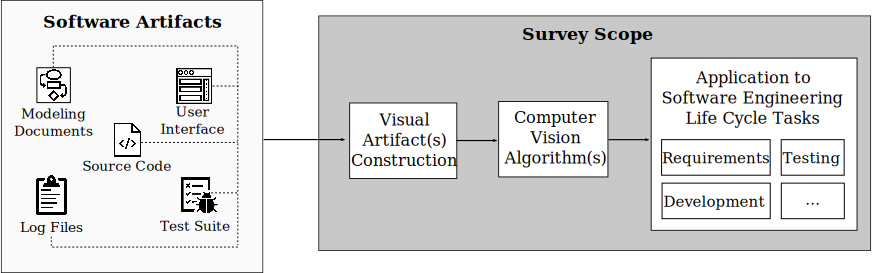
\includegraphics[scale=0.50]{survey/figures/scope-horizontal}
    %}
    \caption{Overview of the scope of this survey.}
    \label{fig:scope}
\end{figure*}




